\documentclass{article}\usepackage[]{graphicx}\usepackage[]{color}
%% maxwidth is the original width if it is less than linewidth
%% otherwise use linewidth (to make sure the graphics do not exceed the margin)
\makeatletter
\def\maxwidth{ %
  \ifdim\Gin@nat@width>\linewidth
    \linewidth
  \else
    \Gin@nat@width
  \fi
}
\makeatother

\definecolor{fgcolor}{rgb}{0.345, 0.345, 0.345}
\newcommand{\hlnum}[1]{\textcolor[rgb]{0.686,0.059,0.569}{#1}}%
\newcommand{\hlstr}[1]{\textcolor[rgb]{0.192,0.494,0.8}{#1}}%
\newcommand{\hlcom}[1]{\textcolor[rgb]{0.678,0.584,0.686}{\textit{#1}}}%
\newcommand{\hlopt}[1]{\textcolor[rgb]{0,0,0}{#1}}%
\newcommand{\hlstd}[1]{\textcolor[rgb]{0.345,0.345,0.345}{#1}}%
\newcommand{\hlkwa}[1]{\textcolor[rgb]{0.161,0.373,0.58}{\textbf{#1}}}%
\newcommand{\hlkwb}[1]{\textcolor[rgb]{0.69,0.353,0.396}{#1}}%
\newcommand{\hlkwc}[1]{\textcolor[rgb]{0.333,0.667,0.333}{#1}}%
\newcommand{\hlkwd}[1]{\textcolor[rgb]{0.737,0.353,0.396}{\textbf{#1}}}%

\usepackage{framed}
\makeatletter
\newenvironment{kframe}{%
 \def\at@end@of@kframe{}%
 \ifinner\ifhmode%
  \def\at@end@of@kframe{\end{minipage}}%
  \begin{minipage}{\columnwidth}%
 \fi\fi%
 \def\FrameCommand##1{\hskip\@totalleftmargin \hskip-\fboxsep
 \colorbox{shadecolor}{##1}\hskip-\fboxsep
     % There is no \\@totalrightmargin, so:
     \hskip-\linewidth \hskip-\@totalleftmargin \hskip\columnwidth}%
 \MakeFramed {\advance\hsize-\width
   \@totalleftmargin\z@ \linewidth\hsize
   \@setminipage}}%
 {\par\unskip\endMakeFramed%
 \at@end@of@kframe}
\makeatother

\definecolor{shadecolor}{rgb}{.97, .97, .97}
\definecolor{messagecolor}{rgb}{0, 0, 0}
\definecolor{warningcolor}{rgb}{1, 0, 1}
\definecolor{errorcolor}{rgb}{1, 0, 0}
\newenvironment{knitrout}{}{} % an empty environment to be redefined in TeX

\usepackage{alltt}
\usepackage{geometry}
\geometry{verbose,tmargin=2cm,bmargin=2cm,lmargin=2.5cm,rmargin=2.5cm}
\IfFileExists{upquote.sty}{\usepackage{upquote}}{}
\begin{document}





\title{WA State HIV Testing Histories - Description of Analysis Sample}
\author{Martina Morris and Jeanette Birnbaum}
\maketitle

\section{Sample Reminder}

\begin{itemize}
    \item N = 4744
    \item Years = 2005 to 2013
    \item everHadNegTest = TRUE for 2116 (44.6\%), FALSE for 589 (12.42\%), and NA for 2039 (42.98\%)
\end{itemize}

\section{Number of Diagnoses}

\begin{knitrout}\footnotesize
\definecolor{shadecolor}{rgb}{0.969, 0.969, 0.969}\color{fgcolor}\begin{kframe}
\begin{verbatim}
## 
##    2005 2005.25  2005.5 2005.75    2006 2006.25  2006.5 2006.75    2007 2007.25 
##     155     129     131     142     129     153     121     135     162     148 
##  2007.5 2007.75    2008 2008.25  2008.5 2008.75    2009 2009.25  2009.5 2009.75 
##     150     119     124     162     126     124     141     140     122     133 
##    2010 2010.25  2010.5 2010.75    2011 2011.25  2011.5 2011.75    2012 2012.25 
##     156     130     137     121     139     112     109     129     138     140 
##  2012.5 2012.75    2013 2013.25  2013.5 2013.75 
##     116     111     123     118     106     113
## [1] 4744
\end{verbatim}
\end{kframe}

{\centering 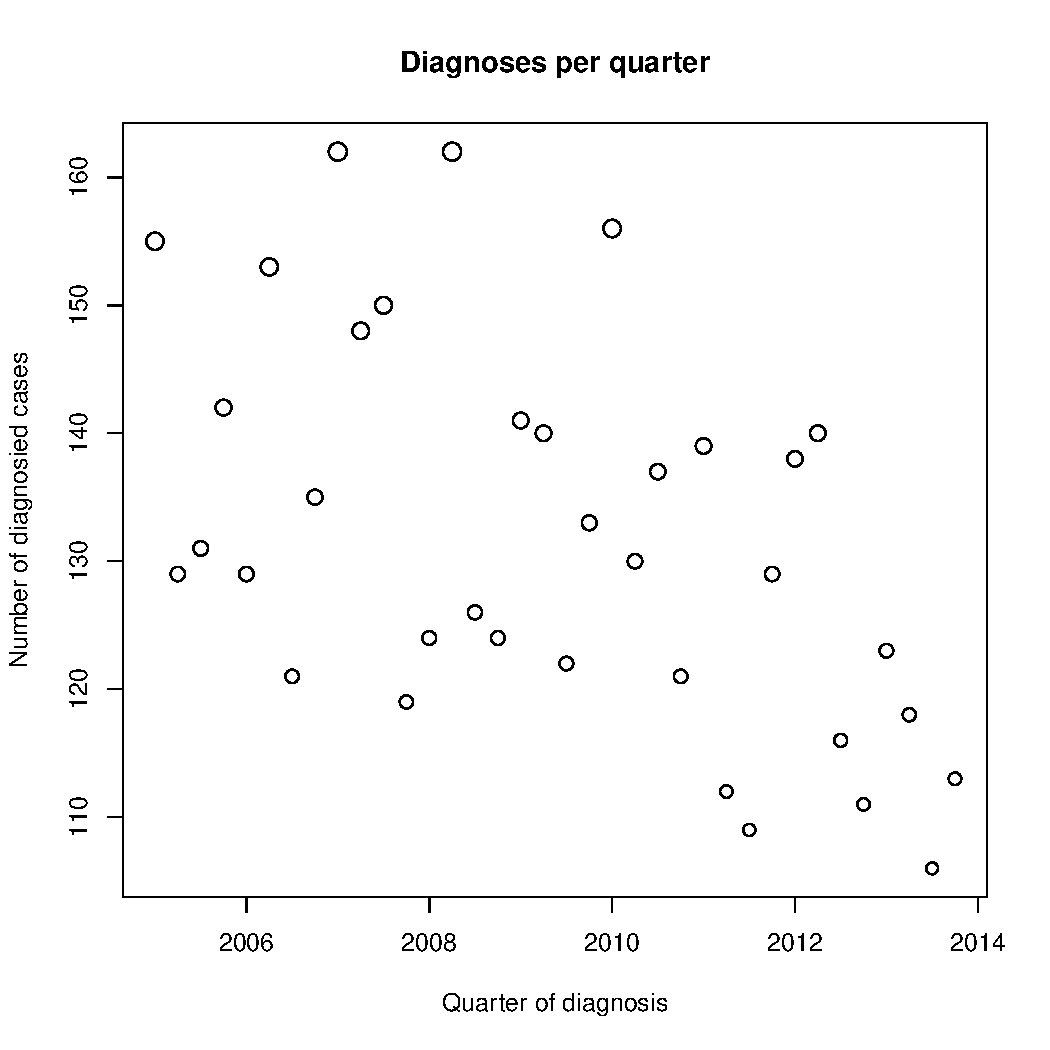
\includegraphics[width=\maxwidth]{figure/minimal-diagnoses} 

}



\end{knitrout}


\section{Age at Diagnosis}

\begin{knitrout}\footnotesize
\definecolor{shadecolor}{rgb}{0.969, 0.969, 0.969}\color{fgcolor}

{\centering 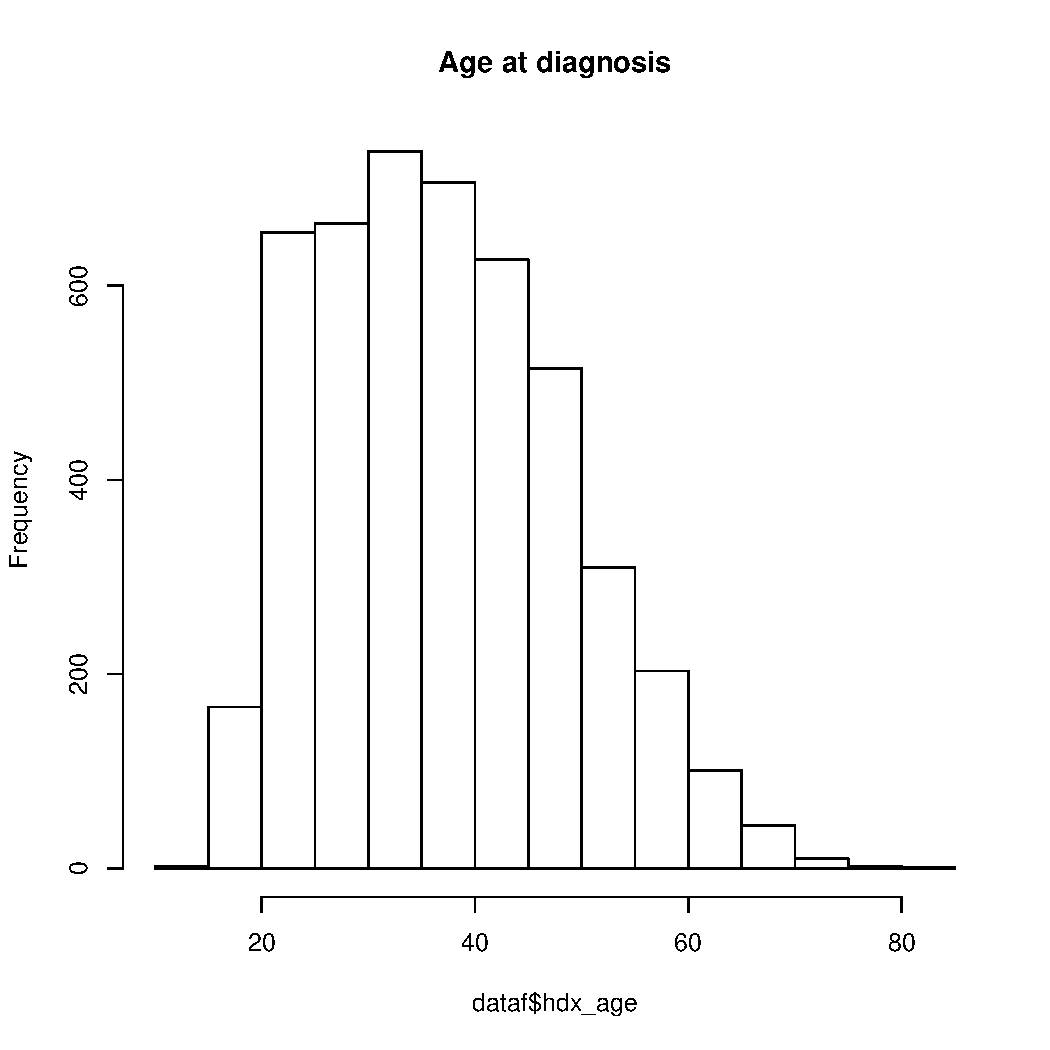
\includegraphics[width=\maxwidth]{figure/minimal-age} 

}



\end{knitrout}


\section{everHadNegTest by subgroups}

\begin{knitrout}\footnotesize
\definecolor{shadecolor}{rgb}{0.969, 0.969, 0.969}\color{fgcolor}\begin{kframe}
\begin{alltt}
\hlcom{############################################################# everHadNegTest}

\hlstd{variables} \hlkwb{<-} \hlkwd{c}\hlstd{(}\hlkwc{`Age Group`} \hlstd{=} \hlstr{"agecat5"}\hlstd{,} \hlkwc{`Race/Ethnicity`} \hlstd{=} \hlstr{"race"}\hlstd{,} \hlkwc{`Mode of Transmission`} \hlstd{=} \hlstr{"mode"}\hlstd{)}

\hlstd{(everHadNegTest_subgrouptab} \hlkwb{<-} \hlkwd{tabulate_everHadNegTest}\hlstd{(dataf, variables,} \hlkwc{supercolumn} \hlstd{=} \hlnum{TRUE}\hlstd{))}
\end{alltt}
\begin{verbatim}
##          Characteristic     Subgroup    N Column.Percent Percent.Yes Percent.No
## 1             Age Group         <=20  168              4          49         18
## 2                              21-25  655             14          54         12
## 3                              26-30  664             14          52         10
## 4                              31-35  738             16          49         10
## 5                              36-40  706             15          41         11
## 6                              41-45  627             13          43         12
## 7                              46-50  515             11          35         12
## 8                              51-55  310              7          35         16
## 9                              56-60  203              4          37         23
## 10                             61-65  101              2          23         21
## 11                             66-70   44              1          34         18
## 12                             71-85   13              0          46         15
## 13       Race/Ethnicity        White 2773             58          50         10
## 14                             Black  792             17          35         16
## 15                              Hisp  732             15          39         13
## 16                             Asian  220              5          30         23
## 17                            Native   95              2          28         24
## 18                             Multi  132              3          50         15
## 19 Mode of Transmission          MSM 3135             66          56         10
## 20                            Hetero 1334             28          22         18
## 21                      Blood/Needle  275              6          29         16
##    Percent.Missing
## 1               33
## 2               34
## 3               38
## 4               41
## 5               48
## 6               46
## 7               52
## 8               48
## 9               40
## 10              56
## 11              48
## 12              38
## 13              40
## 14              49
## 15              48
## 16              47
## 17              47
## 18              35
## 19              35
## 20              60
## 21              55
\end{verbatim}
\begin{alltt}
\hlstd{(everHadNegTest_racebydx} \hlkwb{<-} \hlkwd{tabulate_everHadNegTest}\hlstd{(dataf,} \hlkwd{list}\hlstd{(}\hlkwd{c}\hlstd{(}\hlstr{"mode"}\hlstd{,} \hlstr{"race"}\hlstd{))))}
\end{alltt}
\begin{verbatim}
##            mode   race    N Column Percent Percent Yes Percent No
## 1           MSM  White 2141             45          57          8
## 2           MSM  Black  281              6          55         12
## 3           MSM   Hisp  461             10          54         11
## 4           MSM  Asian  112              2          49         13
## 5           MSM Native   45              1          44         22
## 6           MSM  Multi   95              2          58         16
## 7        Hetero  White  454             10          27         15
## 8        Hetero  Black  476             10          25         17
## 9        Hetero   Hisp  236              5          12         18
## 10       Hetero  Asian  102              2          12         32
## 11       Hetero Native   39              1          10         31
## 12       Hetero  Multi   27              1          26         15
## 13 Blood/Needle  White  178              4          30         16
## 14 Blood/Needle  Black   35              1          29         20
## 15 Blood/Needle   Hisp   35              1          23         17
## 16 Blood/Needle  Asian    6              0           0         33
## 17 Blood/Needle Native   11              0          27          9
## 18 Blood/Needle  Multi   10              0          40         10
##    Percent Missing
## 1               35
## 2               33
## 3               35
## 4               38
## 5               33
## 6               26
## 7               58
## 8               58
## 9               70
## 10              56
## 11              59
## 12              59
## 13              54
## 14              51
## 15              60
## 16              67
## 17              64
## 18              50
\end{verbatim}
\end{kframe}
\end{knitrout}


\section{TID by everHadNegTest}

\begin{knitrout}\footnotesize
\definecolor{shadecolor}{rgb}{0.969, 0.969, 0.969}\color{fgcolor}\begin{kframe}
\begin{verbatim}
## $stats
##   Group Min. 1st Qu. Median   Mean 3rd Qu.  Max. IsNA    N Percent Missing
## 1 FALSE    1 12.0000 17.980 15.010  17.980 17.98    0  589               0
## 2    NA   NA      NA     NA    NaN      NA    NA 2039 2039             100
## 3  TRUE    0  0.4959  1.185  2.515   3.062 17.98    0 2116               0
## 
## $oneway
## 
## 	One-way analysis of means (not assuming equal variances)
## 
## data:  infPeriod and Group
## F = 3647.57, num df = 1.000, denom df = 757.033, p-value < 2.2e-16
\end{verbatim}
\end{kframe}
\end{knitrout}


\section{TID Over Time}

\begin{knitrout}\footnotesize
\definecolor{shadecolor}{rgb}{0.969, 0.969, 0.969}\color{fgcolor}\begin{kframe}
\begin{verbatim}
## $stats
##   Group Min. 1st Qu. Median  Mean 3rd Qu.  Max. IsNA   N Percent Missing
## 1  2005    0  0.5596  1.352 4.210   4.690 17.98  437 557           78.46
## 2  2006    0  0.7082  2.290 5.842   9.590 17.98  275 538           51.12
## 3  2007    0  0.5808  1.808 5.016   6.541 17.98  284 579           49.05
## 4  2008    0  0.8760  2.230 5.334   7.055 17.98  274 536           51.12
## 5  2009    0  0.6795  1.874 4.900   6.410 17.98  205 536           38.25
## 6  2010    0  0.5267  1.933 4.907   6.599 17.98  140 544           25.74
## 7  2011    0  0.7288  2.523 5.267   7.463 17.98  116 489           23.72
## 8  2012    0  0.6740  2.321 5.670   9.729 17.98  148 505           29.31
## 9  2013    0  0.5959  1.953 5.509   9.000 17.98  160 460           34.78
## 
## $oneway
## 
## 	One-way analysis of means (not assuming equal variances)
## 
## data:  infPeriod and Group
## F = 1.308, num df = 8.000, denom df = 971.386, p-value = 0.2355
\end{verbatim}


{\ttfamily\noindent\color{warningcolor}{\#\# Warning: Removed 2039 rows containing non-finite values (stat\_boxplot).\\\#\# Warning: Removed 2039 rows containing missing values (geom\_point).}}\end{kframe}

{\centering 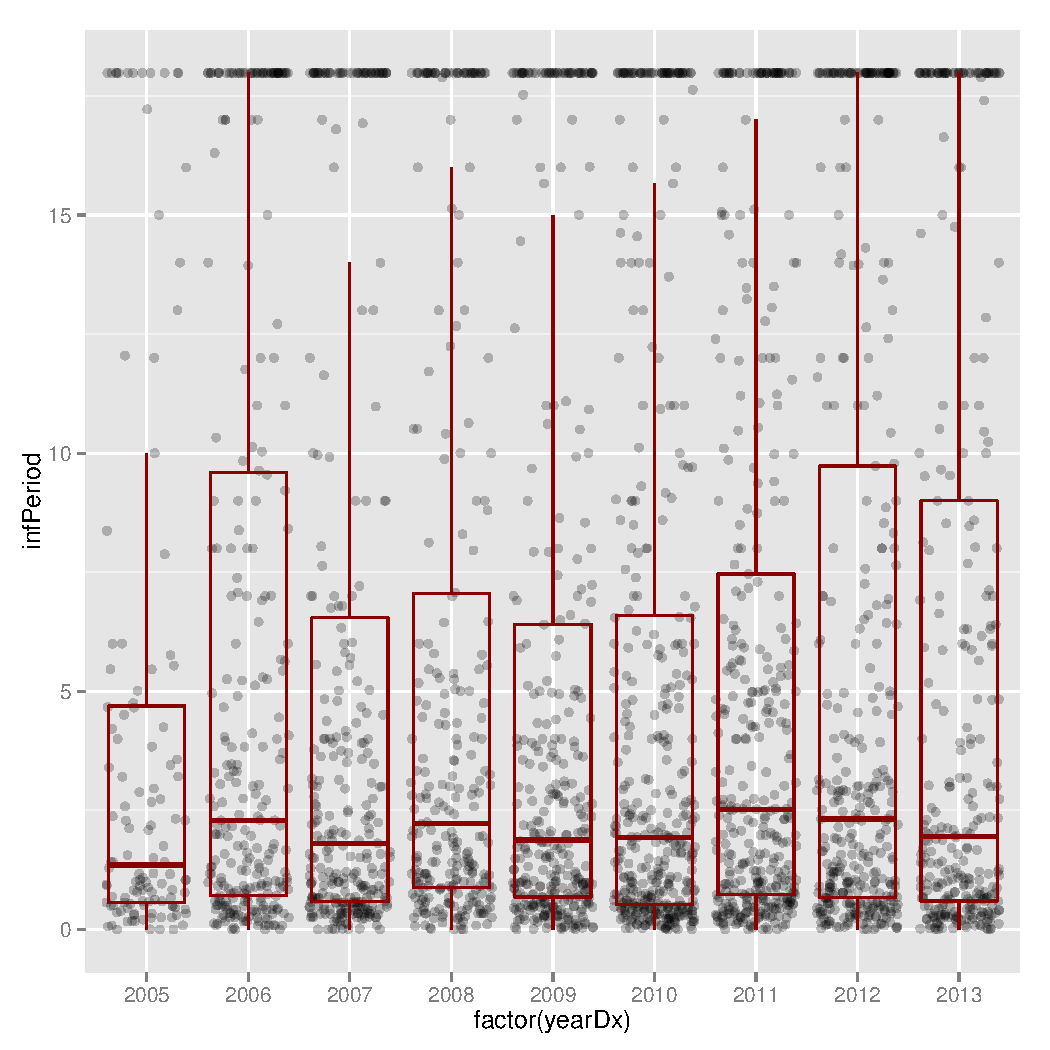
\includegraphics[width=\maxwidth]{figure/minimal-time} 

}



\end{knitrout}


\section{TID by Race}

\begin{knitrout}\footnotesize
\definecolor{shadecolor}{rgb}{0.969, 0.969, 0.969}\color{fgcolor}\begin{kframe}
\begin{verbatim}
## $stats
##   Group    Min. 1st Qu. Median  Mean 3rd Qu.  Max. IsNA    N Percent Missing
## 1 White 0.00000  0.5479  1.716 4.509   5.547 17.98 1109 2773           39.99
## 2 Black 0.00000  0.9863  3.836 7.038  14.000 17.98  387  792           48.86
## 3  Hisp 0.00000  0.6849  2.282 5.667  10.500 17.98  349  732           47.68
## 4 Asian 0.00000  1.0490  4.126 7.450  17.000 17.98  103  220           46.82
## 5 NHoPI 0.01370  0.3616  4.852 7.315  12.750 17.98   13   33           39.39
## 6 AI/AN 0.02466  1.1290  5.189 7.130  10.100 17.98   32   62           51.61
## 7 Multi 0.00000  0.4918  1.693 4.758   6.285 17.98   46  132           34.85
## 
## $oneway
## 
## 	One-way analysis of means (not assuming equal variances)
## 
## data:  infPeriod and Group
## F = 11.1283, num df = 6.000, denom df = 146.815, p-value = 3.258e-10
\end{verbatim}


{\ttfamily\noindent\color{warningcolor}{\#\# Warning: Removed 2039 rows containing non-finite values (stat\_boxplot).\\\#\# Warning: Removed 2039 rows containing missing values (geom\_point).}}\end{kframe}

{\centering 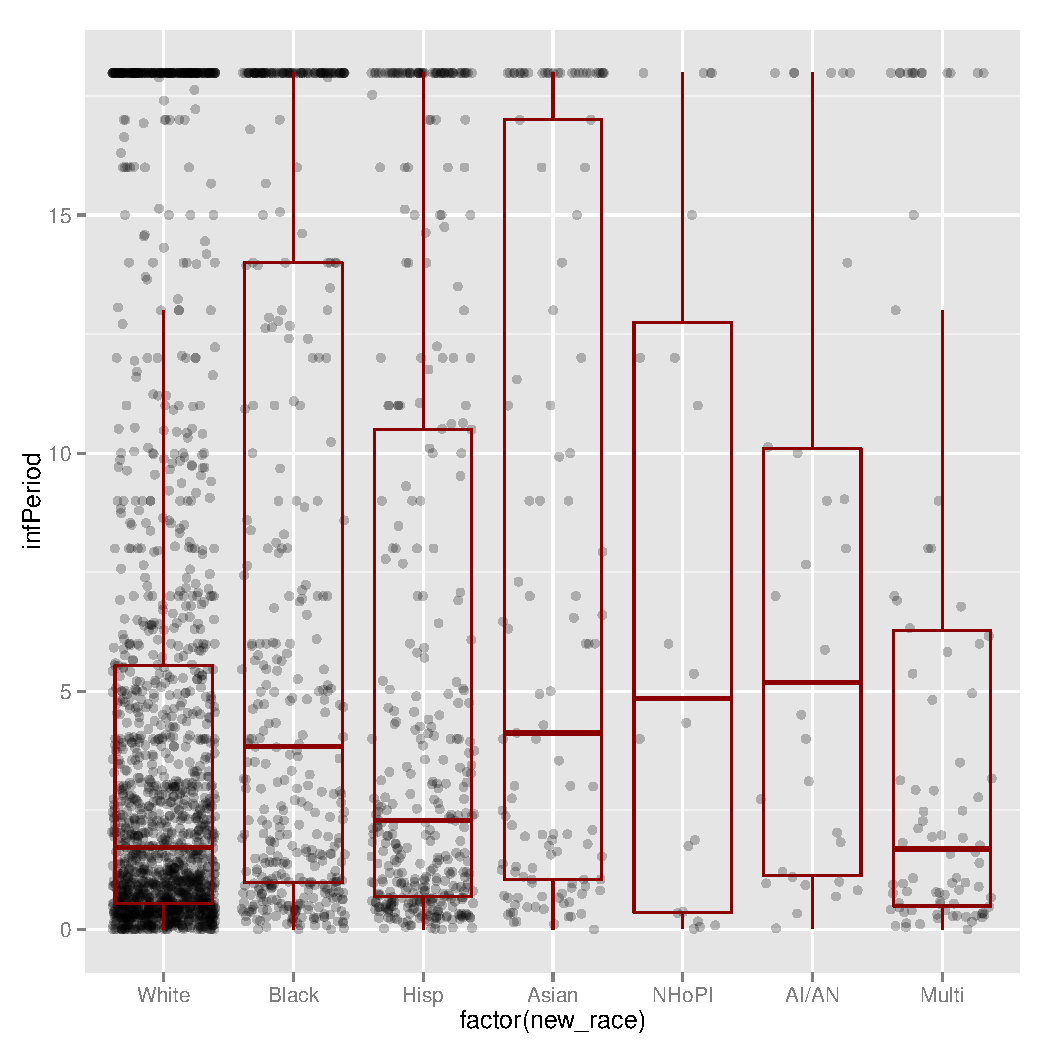
\includegraphics[width=\maxwidth]{figure/minimal-race} 

}



\end{knitrout}


\section{TID by Mode2}

\begin{knitrout}\footnotesize
\definecolor{shadecolor}{rgb}{0.969, 0.969, 0.969}\color{fgcolor}\begin{kframe}
\begin{alltt}
\hlcom{############################################################# MODE2}

\hlkwd{summarize_infPeriod}\hlstd{(dataf}\hlopt{$}\hlstd{infPeriod,} \hlkwc{bygroup} \hlstd{= dataf}\hlopt{$}\hlstd{mode2)}
\end{alltt}
\begin{verbatim}
## $stats
##     Group Min. 1st Qu. Median  Mean 3rd Qu.  Max. IsNA    N Percent Missing
## 1     MSM    0   0.511  1.419 4.002   4.729 17.98 1088 3135           34.70
## 2 non-MSM    0   2.082  6.849 9.078  17.980 17.98  951 1609           59.11
## 
## $oneway
## 
## 	One-way analysis of means (not assuming equal variances)
## 
## data:  infPeriod and Group
## F = 278.1611, num df = 1.000, denom df = 918.046, p-value < 2.2e-16
\end{verbatim}
\begin{alltt}
\hlcom{# MSM vs non-MSM counts and % of all diagnoses}
\hlkwd{table}\hlstd{(dataf}\hlopt{$}\hlstd{mode2)}
\end{alltt}
\begin{verbatim}
## 
##     MSM non-MSM 
##    3135    1609
\end{verbatim}
\begin{alltt}
\hlkwd{table}\hlstd{(dataf}\hlopt{$}\hlstd{mode2)}\hlopt{/}\hlkwd{nrow}\hlstd{(dataf)}
\end{alltt}
\begin{verbatim}
## 
##       MSM   non-MSM 
## 0.6608347 0.3391653
\end{verbatim}
\begin{alltt}
\hlcom{# Missing TID (is.na(infPeriod)) by mode2}
\hlkwd{table}\hlstd{(dataf}\hlopt{$}\hlstd{mode2,} \hlkwd{is.na}\hlstd{(dataf}\hlopt{$}\hlstd{infPeriod))}
\end{alltt}
\begin{verbatim}
##          
##           FALSE TRUE
##   MSM      2047 1088
##   non-MSM   658  951
\end{verbatim}
\begin{alltt}
\hlstd{(missTIDmode2} \hlkwb{<-} \hlkwd{table}\hlstd{(dataf}\hlopt{$}\hlstd{mode2,} \hlkwd{is.na}\hlstd{(dataf}\hlopt{$}\hlstd{infPeriod)))}
\end{alltt}
\begin{verbatim}
##          
##           FALSE TRUE
##   MSM      2047 1088
##   non-MSM   658  951
\end{verbatim}
\begin{alltt}
\hlcom{# % of mode2 cases comprising non-missing TID (is.na=FALSE) and missing}
\hlcom{# (is.na=TRUE)}
\hlstd{missTIDmode2}\hlopt{/}\hlkwd{colSums}\hlstd{(missTIDmode2)}
\end{alltt}
\begin{verbatim}
##          
##               FALSE      TRUE
##   MSM     0.7567468 0.4022181
##   non-MSM 0.3227072 0.4664051
\end{verbatim}
\begin{alltt}
\hlkwd{ggplot}\hlstd{(}\hlkwd{aes}\hlstd{(}\hlkwc{y} \hlstd{= infPeriod,} \hlkwc{x} \hlstd{=} \hlkwd{factor}\hlstd{(mode2)),} \hlkwc{data} \hlstd{= dataf)} \hlopt{+} \hlkwd{geom_jitter}\hlstd{(}\hlkwc{alpha} \hlstd{=} \hlnum{0.25}\hlstd{)} \hlopt{+}
    \hlkwd{geom_boxplot}\hlstd{(}\hlkwc{color} \hlstd{=} \hlstr{"darkred"}\hlstd{,} \hlkwc{fill} \hlstd{=} \hlnum{NA}\hlstd{,} \hlkwc{outlier.size} \hlstd{=} \hlnum{0}\hlstd{)}
\end{alltt}


{\ttfamily\noindent\color{warningcolor}{\#\# Warning: Removed 2039 rows containing non-finite values (stat\_boxplot).\\\#\# Warning: Removed 2039 rows containing missing values (geom\_point).}}\end{kframe}

{\centering 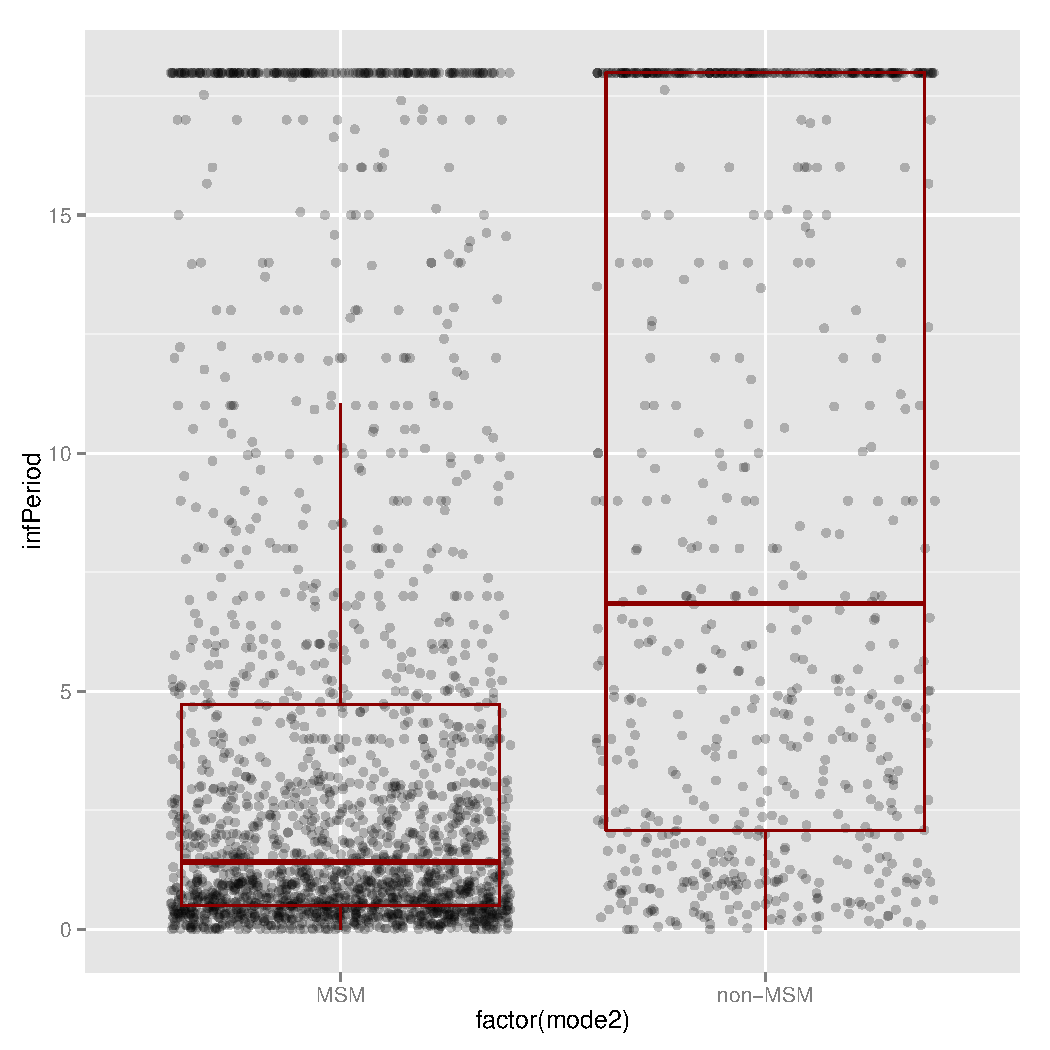
\includegraphics[width=\maxwidth]{figure/minimal-mode2} 

}



\end{knitrout}


\section{TID Density, Upper Bound (Infection at Last Neg Test)}

\begin{knitrout}\footnotesize
\definecolor{shadecolor}{rgb}{0.969, 0.969, 0.969}\color{fgcolor}

{\centering 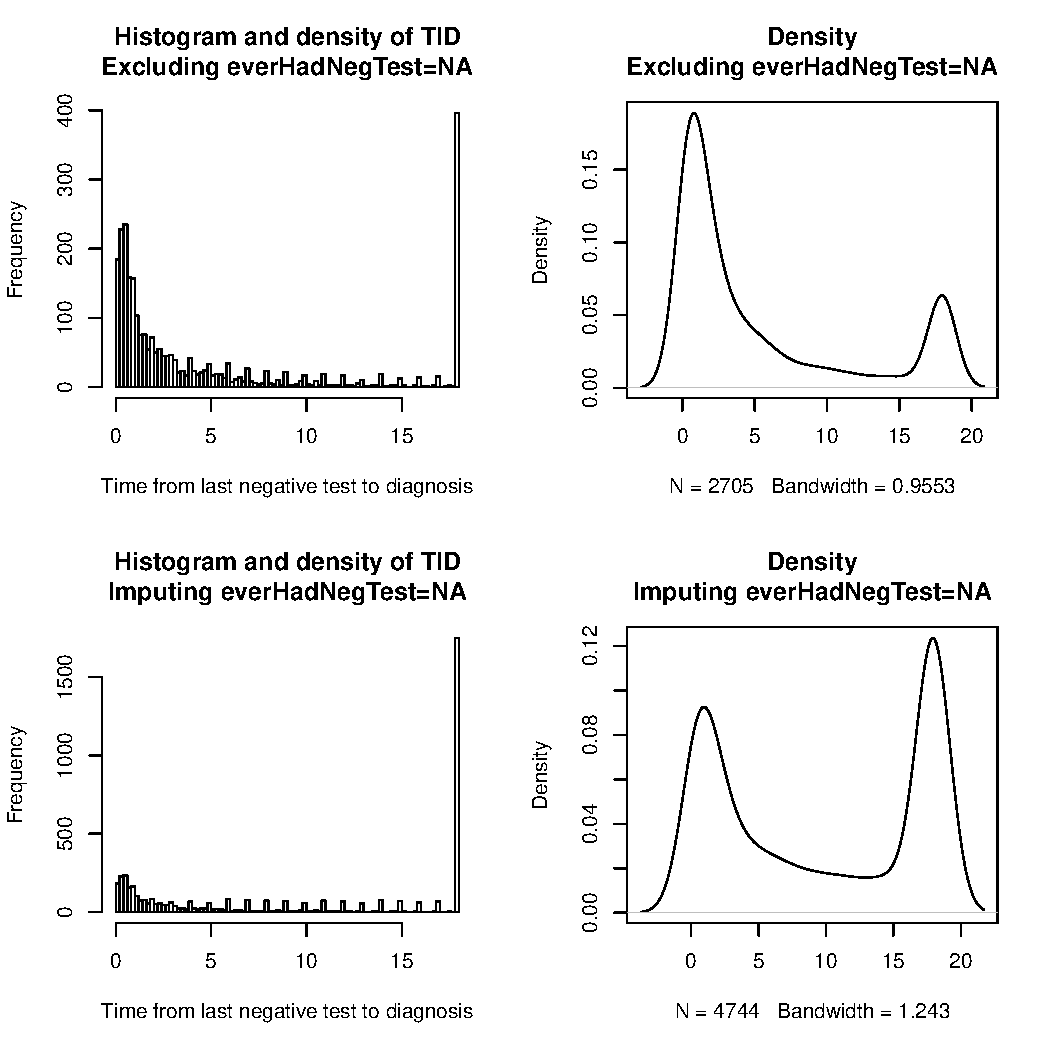
\includegraphics[width=\maxwidth]{figure/minimal-density} 

}



\end{knitrout}


\section{TID Survival Curve, Upper Bound }



\begin{knitrout}\footnotesize
\definecolor{shadecolor}{rgb}{0.969, 0.969, 0.969}\color{fgcolor}

{\centering 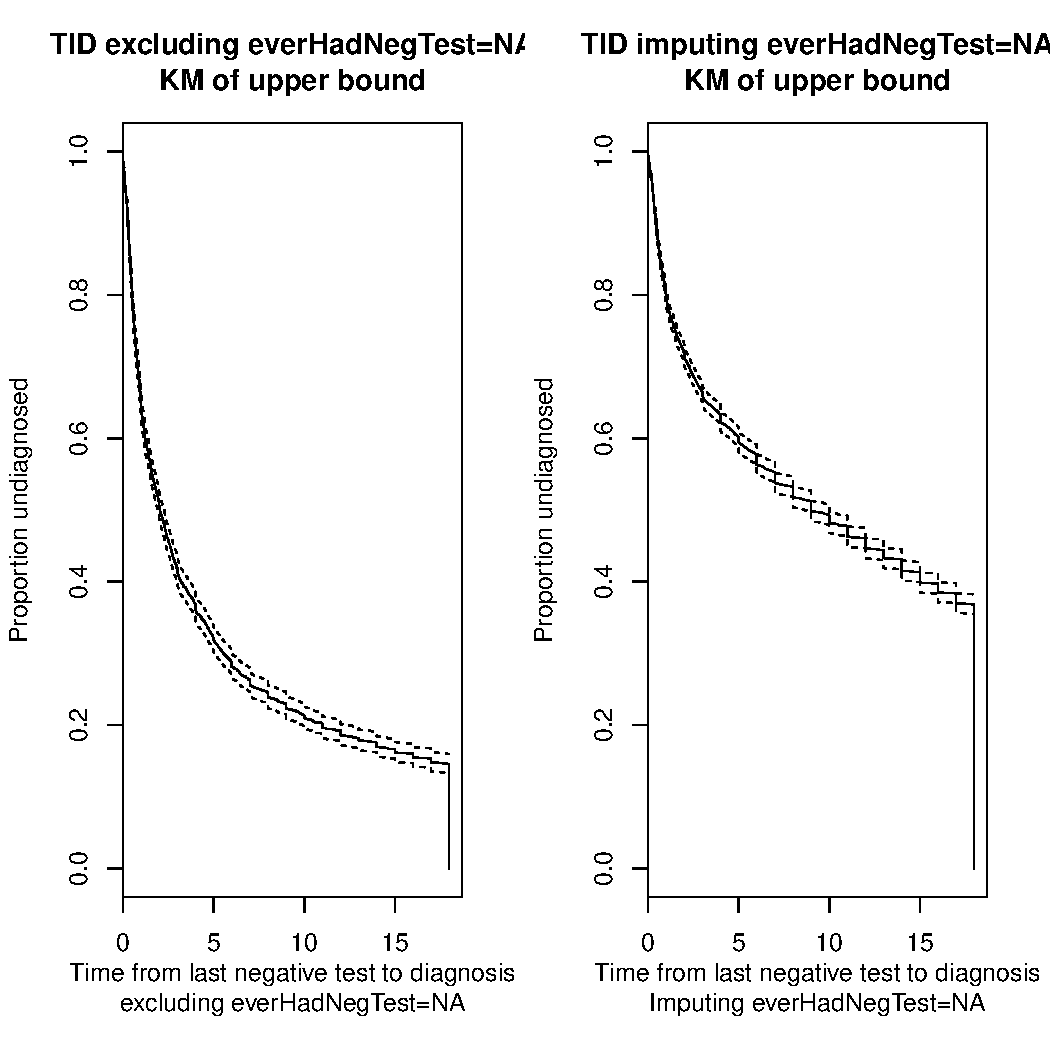
\includegraphics[width=\maxwidth]{figure/minimal-kmplot} 

}



\end{knitrout}


\section{TID Survival Curve, Base Case and Upper Bound}

\begin{knitrout}\footnotesize
\definecolor{shadecolor}{rgb}{0.969, 0.969, 0.969}\color{fgcolor}

{\centering 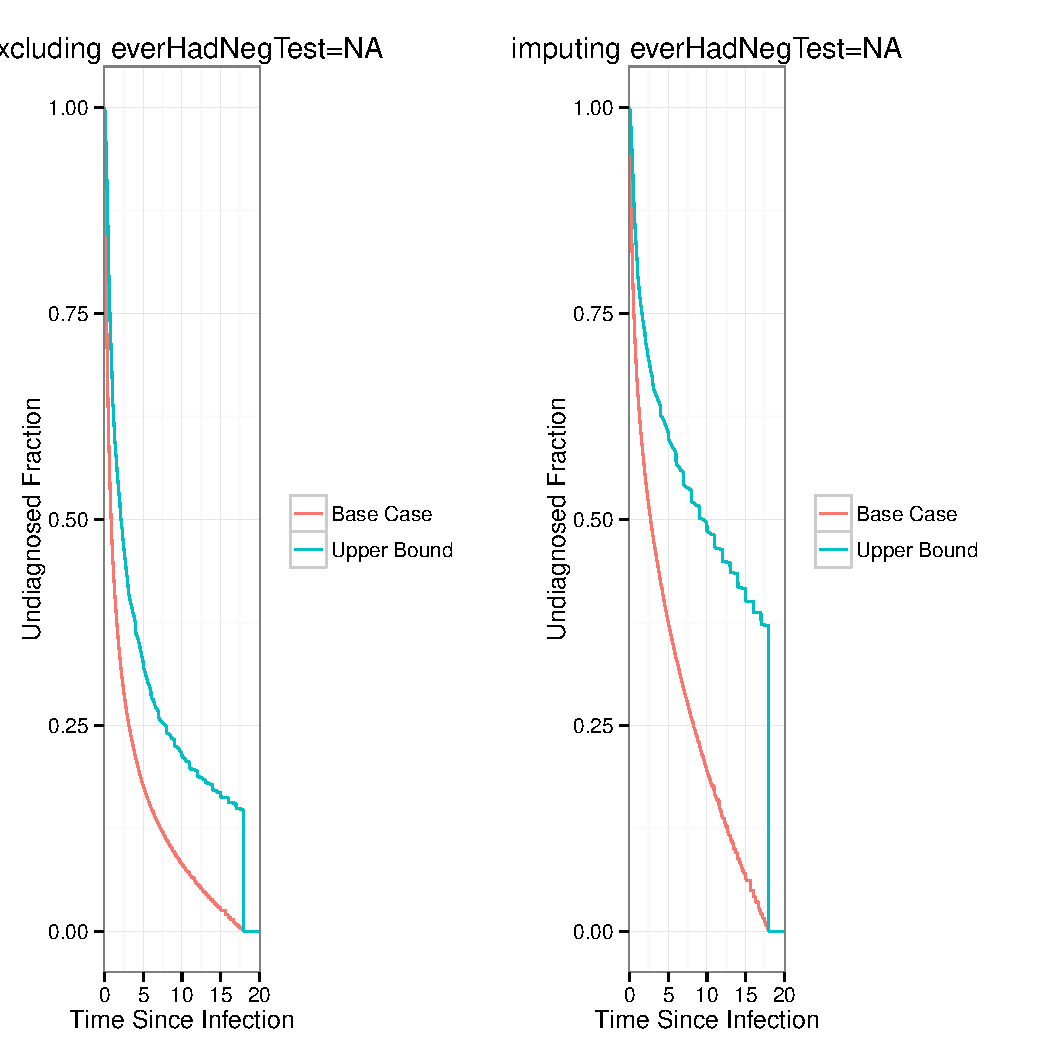
\includegraphics[width=\maxwidth]{figure/minimal-smoothsurv} 

}



\end{knitrout}


\end{document}

